\documentclass[tikz,border=25pt]{standalone}
\usepackage{amsmath,amssymb}
\usetikzlibrary{calc,positioning}

\begin{document}
	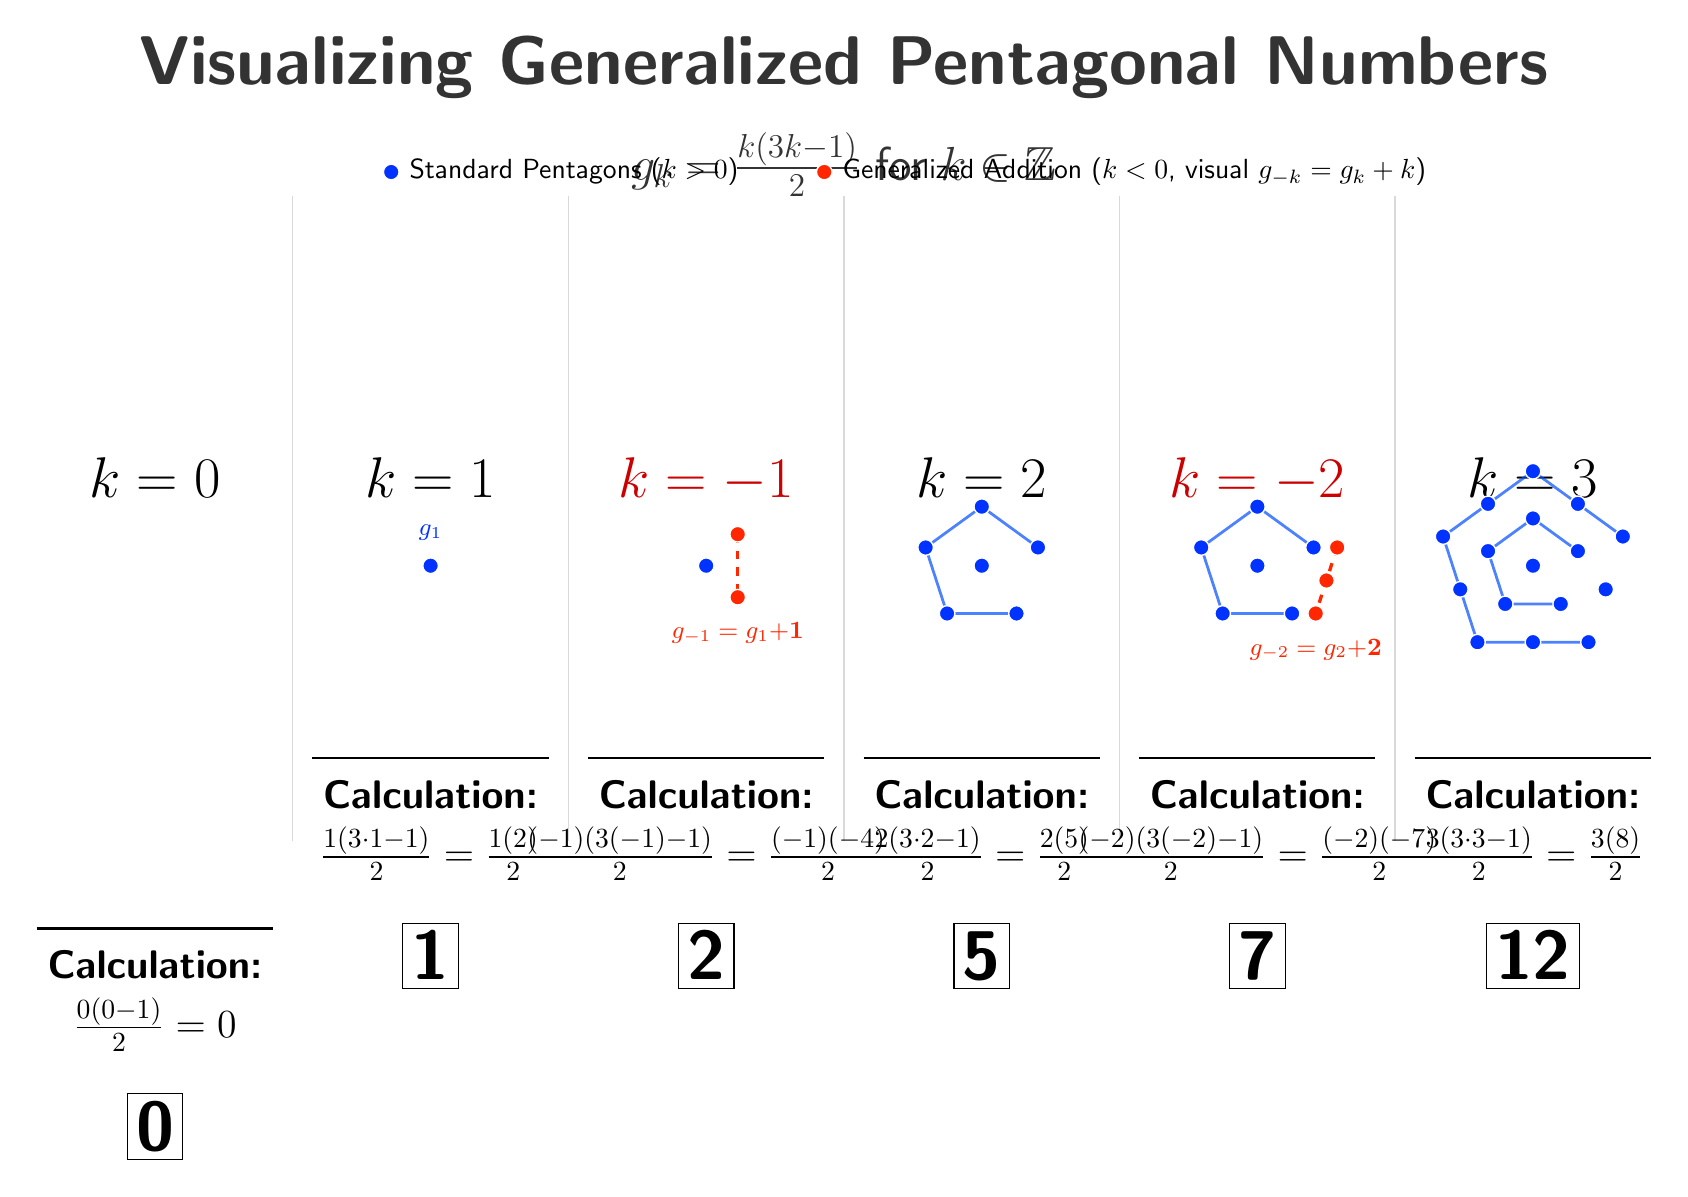
\begin{tikzpicture}[
		font=\sffamily,
		% Dots for the standard pentagons (positive k)
		dot/.style={circle, fill=blue!80!cyan, draw=white, line width=0.5pt, inner sep=2pt},
		% Dots for the extra "bar" in generalized cases (negative k)
		negdot/.style={circle, fill=red!70!orange, draw=white, line width=0.5pt, inner sep=2pt},
		% Lines for edges
		edge/.style={line width=1pt, blue!70!cyan, opacity=0.7},
		negedge/.style={line width=1.2pt, red!70!orange, dashed},
		% Spacer between visual blocks
		spacer/.style={gray!30, line width=0.5pt}
		]
		
		% ==========================================
		% TITLE & LEGEND
		% ==========================================
		\node[align=center, text=black!80] at (8.75, 4.2) {
			{\Huge \textbf{Visualizing Generalized Pentagonal Numbers}} \\[4mm]
			{\LARGE $g_k = \frac{k(3k-1)}{2}$ for $k \in \mathbb{Z}$} % Fixed \ZZ to \mathbb{Z}
		};
		
		% Colored legend dots
		\node[dot, label=right:{Standard Pentagons ($k>0$)}] at (3, 3.5) {};
		\node[negdot, label=right:{Generalized Addition ($k<0$, visual $g_{-k} = g_k + k$)}] at (8.5, 3.5) {};
		
		% Define base coordinates for the 6 segments (k=0 to -3)
		\foreach \i in {0,...,5} {
			\coordinate (Base-\i) at (\i*3.5, 0);
		}
		
		% Draw vertical separator lines
		\foreach \i in {1,...,5} {
			\draw[spacer] ($(Base-\i)+(-1.75, 3.2)$) -- ($(Base-\i)+(-1.75, -5)$);
		}
		
		% ==========================================
		% SEGMENT 1: k = 0
		% ==========================================
		\node[anchor=north, align=center] at (Base-0) {
			{\huge $k = 0$} \\[1.5cm]
			\\[3.15cm] % Placeholder for geometry space
			\rule{3cm}{1pt} \\[2mm] % Fixed \hline
			{\Large \textbf{Calculation:}} \\[2mm]
			{\Large $\frac{0(0-1)}{2} = 0$} \\[5mm]
			\fbox{{\Huge \textbf{0}}}
		};
		% geometry: empty
		
		% ==========================================
		% SEGMENT 2: k = 1
		% ==========================================
		\begin{scope}[shift={(Base-1)}]
			\node[anchor=north] at (0,0) {{\huge $k = 1$}};
			
			% Geometry (P1 = 1)
			\coordinate (v0) at (0, -1.5);
			\node[dot] at (v0) {};
			\node[anchor=south, yshift=2mm, font=\small, text=blue!80!cyan] at (v0) {$g_1$};
			
			% Text
			\node[anchor=north, align=center] at (0, -3.8) {
				\rule{3cm}{1pt} \\[2mm] % Fixed \hline
				{\Large \textbf{Calculation:}} \\[2mm]
				{\Large $\frac{1(3\cdot 1-1)}{2} = \frac{1(2)}{2}$} \\[5mm]
				\fbox{{\Huge \textbf{1}}}
			};
		\end{scope}
		
		% ==========================================
		% SEGMENT 3: k = -1 (P1 + 1 bar)
		% ==========================================
		\begin{scope}[shift={(Base-2)}]
			\node[anchor=north, text=red!80!black] at (0,0) {{\huge $k = -1$}};
			
			% Geometry (P1 base)
			\coordinate (v0) at (0, -1.5);
			\node[dot] at (v0) {};
			
			% Generalized Bar addition (visual length 1, rotated for visual symmetry)
			\coordinate (neg-start) at ($(v0)+(0.4, 0.4)$);
			\coordinate (neg-end)   at ($(v0)+(0.4, -0.4)$);
			
			\draw[negedge] (neg-start) -- (neg-end);
			\node[negdot] at (neg-start) {};
			\node[negdot] at (neg-end) {};
			
			% Legend annotation
			\node[anchor=north, font=\small, text=red!70!orange] at ($(v0)+(0.4, -0.6)$) {$g_{-1} = g_1 \mathbf{+ 1}$};
			
			% Text
			\node[anchor=north, align=center] at (0, -3.8) {
				\rule{3cm}{1pt} \\[2mm] % Fixed \hline
				{\Large \textbf{Calculation:}} \\[2mm]
				{\Large $\frac{(-1)(3(-1)-1)}{2} = \frac{(-1)(-4)}{2}$} \\[5mm]
				\fbox{{\Huge \textbf{2}}}
			};
		\end{scope}
		
		% ==========================================
		% SEGMENT 4: k = 2
		% ==========================================
		\begin{scope}[shift={(Base-3)}]
			\node[anchor=north] at (0,0) {{\huge $k = 2$}};
			
			% Geometry (P2 = 5)
			% Center point (Side length 0)
			\coordinate (c0) at (0, -1.5);
			\node[dot] at (c0) {};
			
			% Define standard Pentagon vertices around it (Side length 1)
			\def\scale{0.75}
			\foreach \a/\n in {18/1, 90/2, 162/3, 234/4, 306/5} {
				\coordinate (v\n) at ($(c0)+(\a:\scale)$);
			}
			% Draw perimeter edges (skipping edges touching origin implicitly)
			\draw[edge] (v1) -- (v2) -- (v3) -- (v4) -- (v5);
			% Draw final dot (overlap)
			\foreach \n in {1,...,5} {\node[dot] at (v\n) {};}
			
			% Text
			\node[anchor=north, align=center] at (0, -3.8) {
				\rule{3cm}{1pt} \\[2mm] % Fixed \hline
				{\Large \textbf{Calculation:}} \\[2mm]
				{\Large $\frac{2(3\cdot 2-1)}{2} = \frac{2(5)}{2}$} \\[5mm]
				\fbox{{\Huge \textbf{5}}}
			};
		\end{scope}
		
		% ==========================================
		% SEGMENT 5: k = -2 (P2 + 2 bar)
		% ==========================================
		\begin{scope}[shift={(Base-4)}]
			\node[anchor=north, text=red!80!black] at (0,0) {{\huge $k = -2$}};
			
			% Geometry (P2 base)
			\coordinate (c0) at (0, -1.5);
			\node[dot] at (c0) {};
			\def\scale{0.75}
			\foreach \a/\n in {18/1, 90/2, 162/3, 234/4, 306/5} {
				\coordinate (v\n) at ($(c0)+(\a:\scale)$);
			}
			\draw[edge] (v1) -- (v2) -- (v3) -- (v4) -- (v5);
			\foreach \n in {1,...,5} {\node[dot] at (v\n) {};}
			
			% Generalized Bar addition (P2 + 2 dots)
			% We add a bar along the 'right' edge vector, defined by v1 and v5
			\coordinate (neg-base) at ($(v1)+(0.3, 0)$);
			\coordinate (neg-v1) at ($(neg-base)+(v1)-(v1)$); % Align to top of edge
			\coordinate (neg-v2) at ($(neg-base)+(v5)-(v1)$); % Align to bottom of edge
			
			\draw[negedge] (neg-v1) -- (neg-v2);
			\node[negdot] at (neg-v1) {};
			\node[negdot] at ($(neg-v1)!0.5!(neg-v2)$) {}; % mid-dot
			\node[negdot] at (neg-v2) {};
			
			% Legend annotation
			\node[anchor=north, font=\small, text=red!70!orange] at ($(neg-v2)+(0, -0.2)$) {$g_{-2} = g_2 \mathbf{+ 2}$};
			
			% Text
			\node[anchor=north, align=center] at (0, -3.8) {
				\rule{3cm}{1pt} \\[2mm] % Fixed \hline
				{\Large \textbf{Calculation:}} \\[2mm]
				{\Large $\frac{(-2)(3(-2)-1)}{2} = \frac{(-2)(-7)}{2}$} \\[5mm]
				\fbox{{\Huge \textbf{7}}}
			};
		\end{scope}
		
		% ==========================================
		% SEGMENT 6: k = 3
		% ==========================================
		\begin{scope}[shift={(Base-5)}]
			\node[anchor=north] at (0,0) {{\huge $k = 3$}};
			
			% Geometry (P3 = 12)
			% Center point
			\coordinate (c0) at (0, -1.5);
			\node[dot] at (c0) {};
			
			% Define side length 1 vertices
			\def\scaleOne{0.6}
			\foreach \a/\n in {18/1, 90/2, 162/3, 234/4, 306/5} {
				\coordinate (vOne\n) at ($(c0)+(\a:\scaleOne)$);
			}
			\draw[edge] (vOne1) -- (vOne2) -- (vOne3) -- (vOne4) -- (vOne5);
			
			% Define side length 2 vertices (scale doubled)
			\def\scaleTwo{1.2}
			\foreach \a/\n in {18/1, 90/2, 162/3, 234/4, 306/5} {
				\coordinate (vTwo\n) at ($(c0)+(\a:\scaleTwo)$);
			}
			\draw[edge] (vTwo1) -- (vTwo2) -- (vTwo3) -- (vTwo4) -- (vTwo5);
			
			% Add mid-dots along side-length-2 edges (except overlap vectors)
			% Edge vTwo1 -> vTwo2
			\node[dot] at ($(vTwo1)!0.5!(vTwo2)$) {};
			% Edge vTwo2 -> vTwo3
			\node[dot] at ($(vTwo2)!0.5!(vTwo3)$) {};
			% Edge vTwo3 -> vTwo4
			\node[dot] at ($(vTwo3)!0.5!(vTwo4)$) {};
			% Edge vTwo4 -> vTwo5
			\node[dot] at ($(vTwo4)!0.5!(vTwo5)$) {};
			% Edge vTwo5 -> vTwo1
			\node[dot] at ($(vTwo5)!0.5!(vTwo1)$) {};
			
			% Final overlaps
			\foreach \n in {1,...,5} {\node[dot] at (vOne\n) {};}
			\foreach \n in {1,...,5} {\node[dot] at (vTwo\n) {};}
			
			% Text
			\node[anchor=north, align=center] at (0, -3.8) {
				\rule{3cm}{1pt} \\[2mm] % Fixed \hline
				{\Large \textbf{Calculation:}} \\[2mm]
				{\Large $\frac{3(3\cdot 3-1)}{2} = \frac{3(8)}{2}$} \\[5mm]
				\fbox{{\Huge \textbf{12}}}
			};
		\end{scope}
		
	\end{tikzpicture}
\end{document}